%%% Preamble
\documentclass[paper=a4, fontsize=11pt]{scrartcl}
\usepackage[T1]{fontenc}
\usepackage{fourier}

\usepackage[english]{babel}															% English language/hyphenation
\usepackage[protrusion=true,expansion=true]{microtype}	
\usepackage{amsmath,amsfonts,amsthm} % Math packages
%images and colors
\usepackage{graphicx}
\usepackage{float}

\usepackage{url}
\usepackage{hyperref}
\usepackage[colorinlistoftodos,prependcaption,textsize=tiny]{todonotes}

%%% Custom sectioning
\usepackage{sectsty}
\allsectionsfont{\centering \normalfont\scshape}


%%% Custom headers/footers (fancyhdr package)
\usepackage{fancyhdr}
\pagestyle{fancyplain}
\fancyhead{}											% No page header
\fancyfoot[L]{}											% Empty 
\fancyfoot[C]{}											% Empty
\fancyfoot[R]{\thepage}									% Pagenumbering
\renewcommand{\headrulewidth}{0pt}			% Remove header underlines
\renewcommand{\footrulewidth}{0pt}				% Remove footer underlines
\setlength{\headheight}{13.6pt}


%%% Equation and float numbering
\numberwithin{equation}{section}		% Equationnumbering: section.eq#
\numberwithin{figure}{section}			% Figurenumbering: section.fig#
\numberwithin{table}{section}				% Tablenumbering: section.tab#


%%% Maketitle metadata
\newcommand{\horrule}[1]{\rule{\linewidth}{#1}} 	% Horizontal rule

\title{
		%\vspace{-1in} 	
		\usefont{OT1}{bch}{b}{n}
		\normalfont \normalsize \textsc{Universit\'e Libre de Bruxelles} \\ [25pt]
		\horrule{0.5pt} \\[0.4cm]
		\huge Formal verification of computer systems \\
		\normalsize Traffic Light Model Checker
		\horrule{2pt} \\[0.5cm]
}
\author{
		\normalfont 								\normalsize
        DESCLEFS Maxime, GERARD Pierre, HEREMAN Nicolas,
 MOULART Walter, SCHEMBRI Julian\\[-3pt]		\normalsize
 \today
}
\date{}

%%% Begin document
\begin{document}
\maketitle
\begin{center}

\includegraphics[scale = 1]{picture/ulb.png}
\end{center}
\newpage
\tableofcontents
\newpage
\section{Introduction}
In this section, we are going to discuss about the goal of the project, the different component used, the assumptions made, and the chosen model.

\subsection{Project}

We decided to join the Embedded systems design project and the Formal verification of computer systems because they follow the same idea and we believe the two classes to be complementary and thus doing a merged project will allows us to study all side of the project, from a model to an implementation trough verification.

The goal of the project we choose is to design and implement an embedded system which is a controlled crossroad traffic light system. Some hypothesis regarding the crossroad properties were made and will be explain more deeply in the following sections.

For the embedded project, we modelized an environment, and generated a controller based on that model to avoid unwanted situations through winning strategies, all computed with timed games. 

For the formal verification course, a more formal approach was taken. We also had to modelize the system, but also to verify that the model was compliant to some specific properties. 

\subsection{Hypothesis}

We first had to choose which crossroad will be our template. We strongly took inspiration from the Fraiteur crossroad (Boulevard du triomphe and Beaulieulaan) near Delta metro station. The result of our brainstorming is as follows :

\begin{figure}[!ht] \label{fig:crossroad}
  \centering
    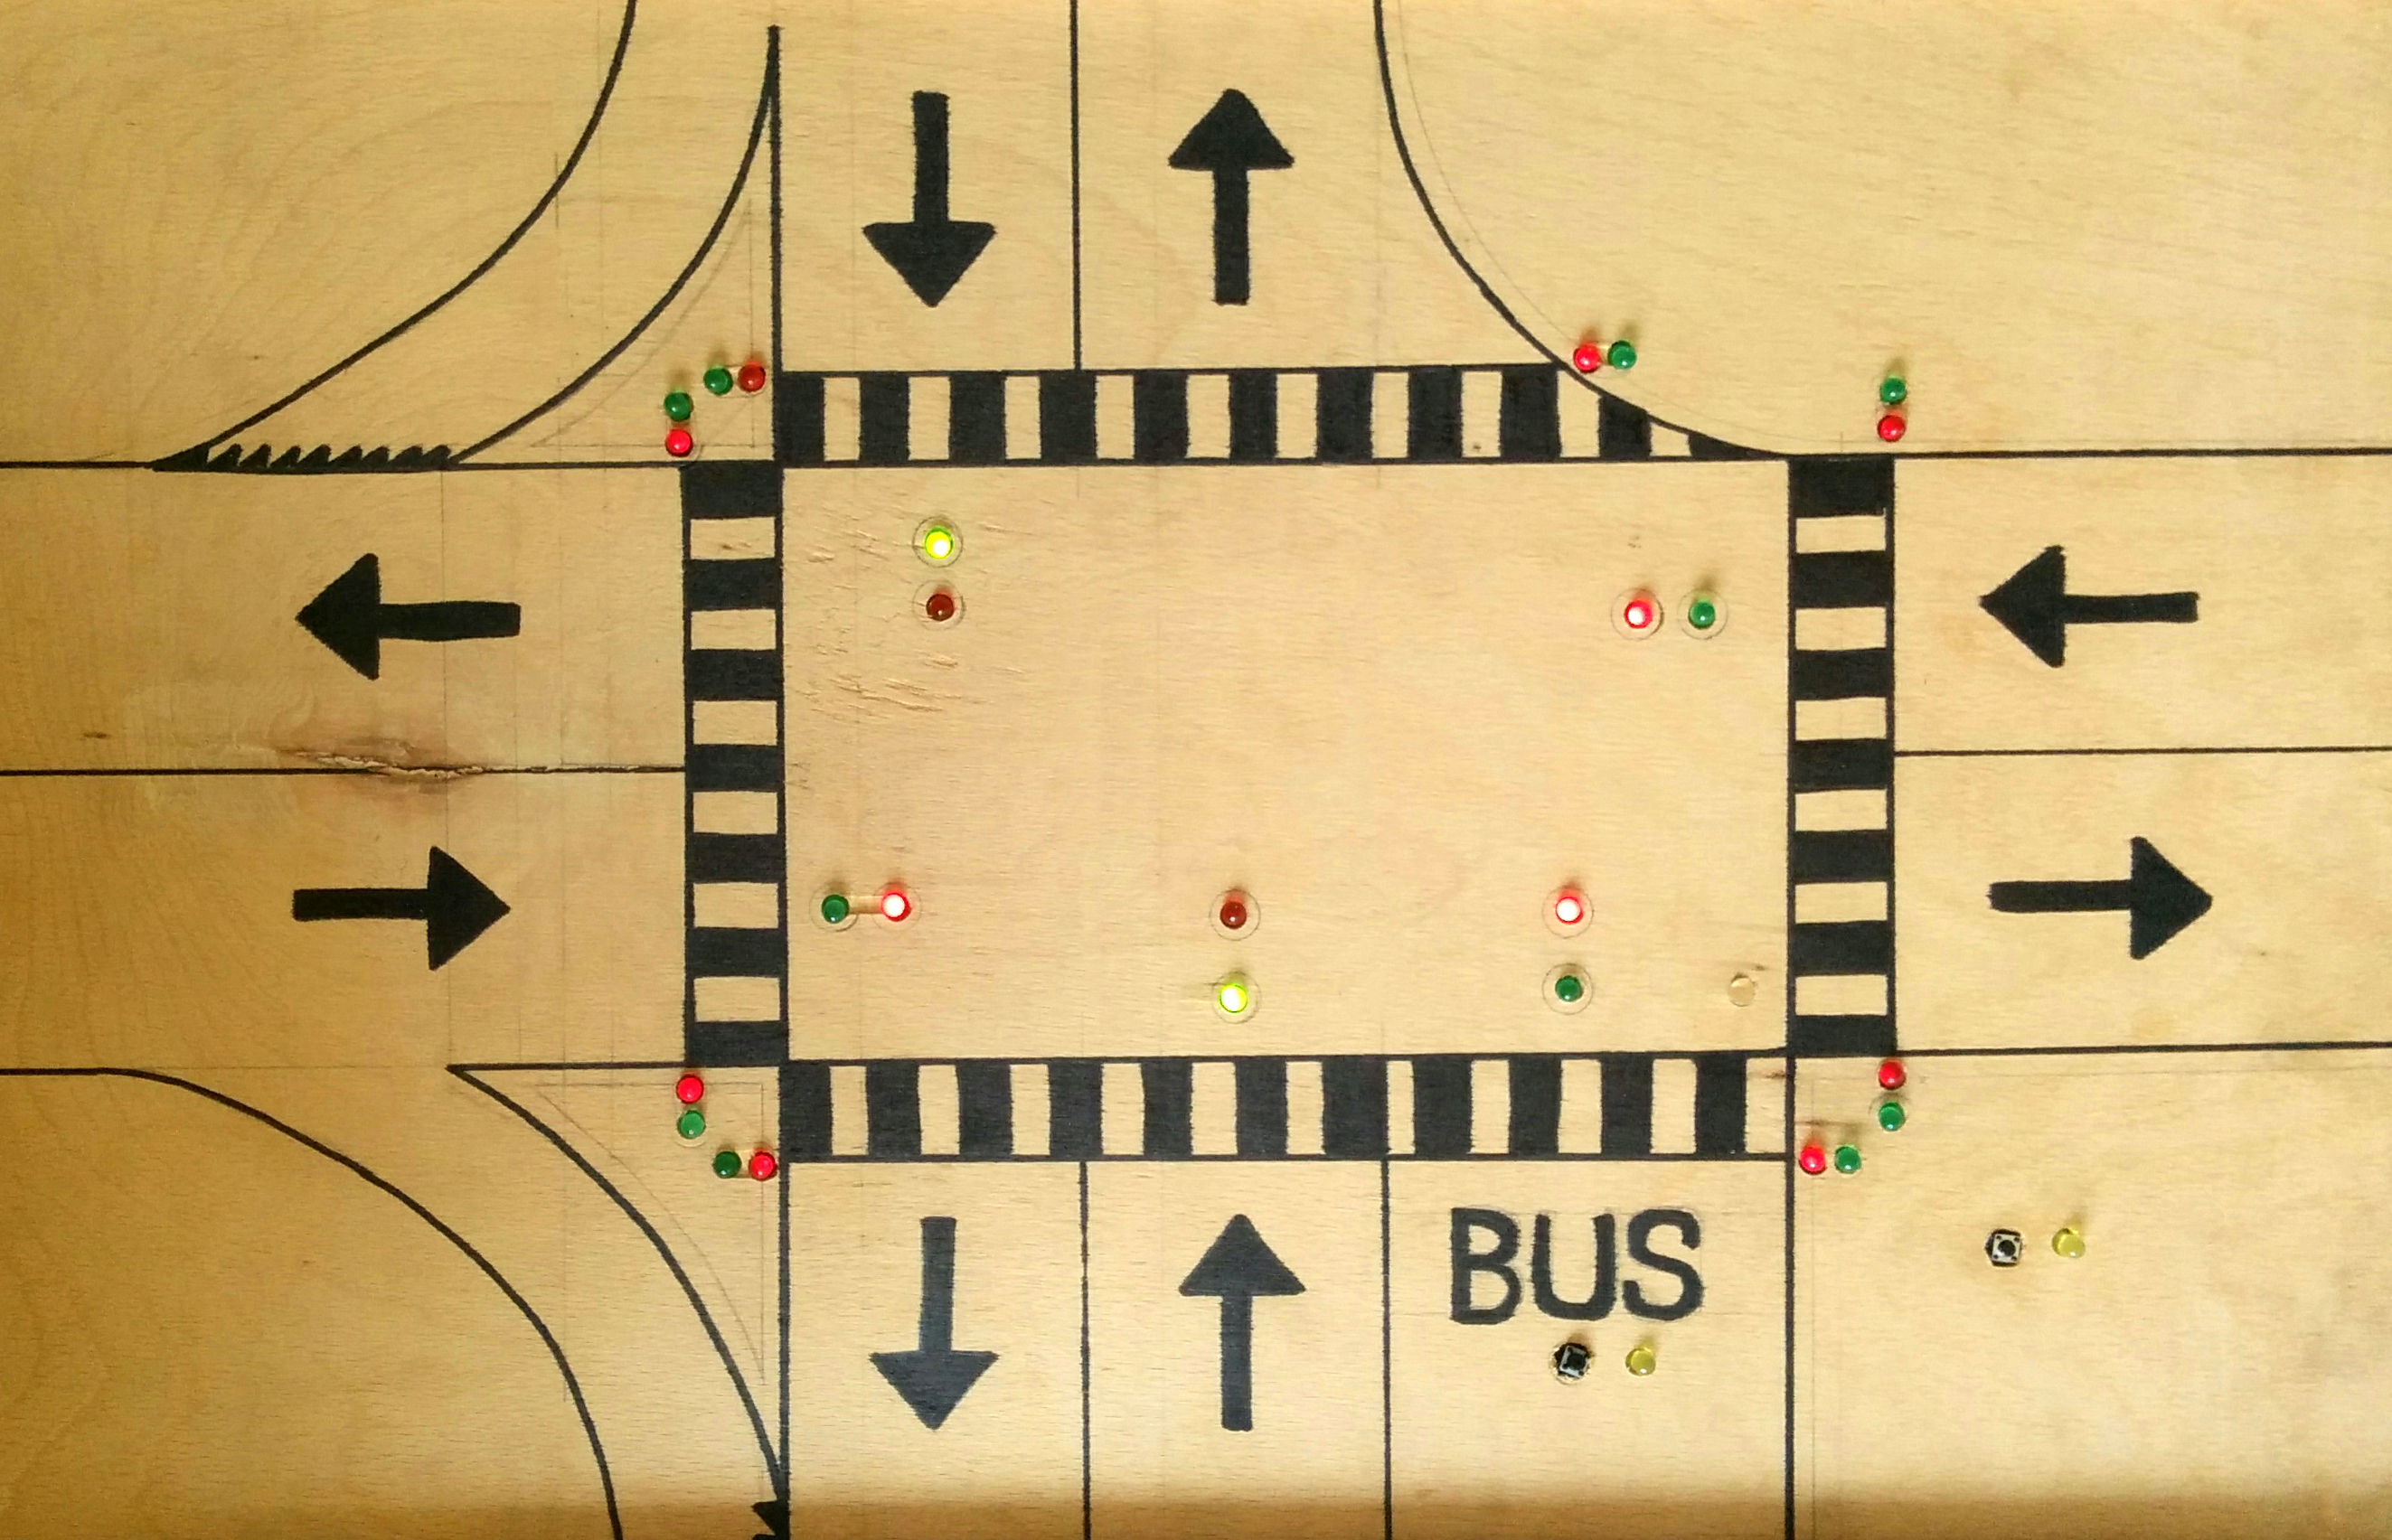
\includegraphics[width=0.75\textwidth]{../common/images/wood-crossroad.jpg}
    \caption{The crossroad model chosen}
\end{figure}

Before defining the different actors and components in our system, some important hypothesis about our model were made:
\begin{itemize}
    \item The different vehicles will respect the Highway Code. This for example means that if a car is turning left and there are car on the opposite direction going straight, the car will stop to let the other pass and will turn after.
    \item At any time, a pedestrian can push a button to cross the street. There is no priority for pedestrian that would push the button many times in a row.
    \item The pedestrians will cross the street within the given time. This also means that they follow the laws and rules.
    \item All the pedestrians light are connected, that means that when pedestrian can cross, all other lights are red.
    \item As for the pedestrians, the vehicles will also cross the street within a given time.
    \item A bus can arrive at any time.
    \item If there is a bus and a pedestrian arriving at the same time, the bus call take the upper hand.
\end{itemize}

\subsection{Actors}
In this section, the different actors interacting with the system will be reviewed. Those include pedestrians, buses and traffic lights.

\subsubsection{Pedestrians}
As shown on Figure \ref{fig:crossroad}, there are four different crosswalks in our model. To make a call for the pedestrians to cross, a push button has been implemented on the controller. This means that when one pedestrian has pushed one of the button of the crossroad, the call has been made for all the pedestrians from all  sides. When the call is accepted by the system, the pedestrians can walk freely in the crossroad. All the lights for the cars and the buses are to be red. This also means that if no pedestrians are pushing the button, meaning that no pedestrians are present, their traffic lights will always be red and the cars are able to drive through the crossroad.
To summarize, when the pedestrians can cross, no other vehicles can. 

\subsubsection{Buses}
The buses in our model can only go from the south path of the crossroad to the west part of it. Those buses will be automatically detected. A bus have a priority on others actors including pedestrians. This means that when a bus cross, and because it has to go through all the others lanes, all others traffic lights have to be red.

\subsubsection{Traffic Lights}
In our Arduino embedded systems, traffic lights can be green or red. We purposely remove the orange light from a common belgian crossroad model because it allows us to avoid having too much cables and LEDs. We consider that when a traffic light is green, cars are going through the crossroad and respect the Highway Code. Therefore cars are not really an actor in our model, we just assume them to pass through the crossroad when their traffic lights are green. 

We want fairness in our system. So for example, even if the pedestrians can always push the button to have the ability to walk through the crosswalk, they have to wait at least that all other traffic lights for the cars have been green once between having two green light. This means that, if no buses come and pedestrians are always pushing the button, the crosswalk with allow the cars of each side to go trough once before the pedestrians can cross again. Thanks to that, each elements in the model can't have only consecutive red light.

Another assumption is, like in common belgian crossroad, that when the South light is green, the North light is also green. On the contrary, when the East light is green, the West light is green. In other words, this means that South-North and East-West direction will have synchronized lights.


\subsection{Arduino}

To test our critical system on a real life environment, we decided to implement it with an arduino, leds and button.

We believe it to be a nice "real-life" exercice because first, for most of us, it was the first time we build something using a micro-controller. Then as we witness it, micro-controller are subject to external unwanted event, like a inducted current in a cable or a button with a badly made pull-up resistor that create an event that should not have taken place. That forces us to create a strong system that can handle all of that.

\section{Concepts}
In this section, important theoretical concepts will be explained using a simple traffic light example because they must be clearly understood in order to ensure that our project reach the required level of success. We will discuss about timed automata, temporal logic and their properties, and game theory to reach a winning condition.

\subsection{Timed Automata} \label{sec:automate}
A timed automaton is essentially a finite automaton (that is a graph
containing a finite number of nodes and labeled edges) extended with real-valued variables. Those automata run on an infinite words as input and they accept timed languages. The variables that exist in the model can represent logical clocks of the system that will be increased synchronously with the same rate.
It is possible to add constraints called \textbf{guards} on the edges to create restriction on our automaton. A transition could thus occur when the value of the clock satisfy the guard's condition on the edge.

\begin{figure}[H]\label{fig:timed}
  \centering
    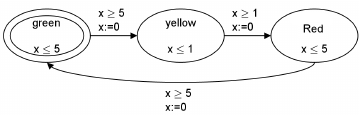
\includegraphics[width=0.7\textwidth]{picture/trafficlight.png}
    \caption{A timed automaton example}
\end{figure}

The example of Figure \ref{fig:timed} represent a basic light example where the light goes from the green state to the yellow state if the clock is higher or equal than 5. It then reset the clock to 0 and stays in the yellow state for a time lower or equal to one. When the clock has an higher value, it switches to the red state and so on.

\subsection{Temporal Logic and Properties}
The aim of temporal logic is to become a formalism of specification and verification of some properties in reactive systems. In our case, two different kind of logic will be of interest: \textbf{Linear Temporal Logic (LTL)} and \textbf{Computation Tree Logic (CTL)}. Those two kind of logic are only concerned with infinite paths. They for example allow us to make statements, such as "Tomorrow, something will eventually be true", something that was not possible with first order logic. Thanks to this, we can define specific properties our system has to comply to. \\
There are of course differences between the two. In the first kind of logic, the LTL one, we will look at the traces of executions, meaning that we will look at the states we reach in a linear manner.
If we look back at Figure \ref{fig:timed}, the traces would be:\\ ${Green \rightarrow Yellow \rightarrow Red \rightarrow Green \rightarrow Yellow \rightarrow Red \rightarrow Green \rightarrow ...}$. \\
In the other kind of logic, the CTL one, we will use a branching time semantic instead of a linear semantic. Here, the different execution (or computation) trees will be considered for all branching possibilities. \\
An example of propriety we can verify thanks to CTL and that is not possible to verify in LTL is "do all executions always have the possibility to eventually reach a certain state". Indeed, intuitively it would require branching to verify it. \\
The following temporal properties can be expressed using either CTL or LTL:
\begin{itemize}
    \item Safety: The system never reaches an unwanted state,
    \item Liveness: Ensure that our system will reach a certain state infinitely often, meaning that no deadlocks can occur,
    \item Persistence: Ensure that a property eventually holds forever,
    \item Fairness: Everyone is at some point satisfied.
\end{itemize}

\subsection{Game Theory and Timed Games} \label{sec:game}
Game theory can be defined as the formal study of decision-making where several players must make choices that potentially affect the interests of the other players\footnote{\url{http://www.cdam.lse.ac.uk/Reports/Files/cdam-2001-09.pdf}}. As when playing a game, we would want to find a winning situation. In our case, there will be two different type of players. The first one will be the controller, something that we can control and define, while the second one, his opponent thus, will be called the environment. \\

The traffic lights will be the first player (the controller since we can control it) while the buses and the pedestrians will be the second player. Since the buses and pedestrians are playing when an external event occurs (a button that is pushed), they will be the environment. The main goal of the controller will be to find a winning strategy in this game, being a sequence of moves that will inevitably lead to the wanted outcome. In our case, we would want the lights to respect the properties that we have defined, even when pedestrians want to cross the street or buses want to go through the crossroad. If at some point all the traffic lights for the cars are green, it would mean that the system is broken and that the controller has lost the game. This is a situation we would not want to happen. \\

\textbf{Times Games} is an important part of the game and the rules, it brings a real-time dimension. An example of a timed game can be a chess game, where each player has to make a move within a given time. In our case, the controller that is the traffic light has to keep the buses, the cars and the pedestrians safe while taking into account the time constraints on the traffic lights.

\section{Tools}
In this section, we will describe the tools used to create our system.

\subsection{UPPAAL}
Uppaal is a tool box for validation (via graphical simulation) and verification (via automatic model-checking) of real-time systems. The idea is to model a system using timed automata, as defined in Section \ref{sec:automate}, simulate it and then verify properties that we can define on it. Those automata will be synchronized through channels. Because Uppaal is based on timed automata, clocks will be an important thing in this software. Indeed, the time will be handle thanks to those clocks. We will see that it will be possible to test the value of a clock or even to reset it. Also, clocks will progress in the whole system at the same time.
\begin{figure}[H]\label{fig:uppaal}
  \begin{center}
    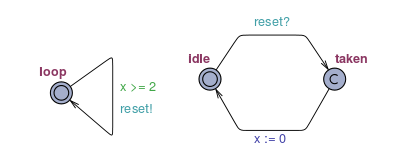
\includegraphics[width=0.8\textwidth]{picture/uppaal.png}
    \caption{Basic example made with UPPAAL}
  \end{center}
\end{figure}
 In Figure \ref{fig:uppaal}, two different elements can be seen. On the left part, there is a loop that will, when the clock x is higher or equal to 2, trigger a reset transition. On the right part, we have a system that wait for a reset. When the trigger has been done by the left component, it is send to the right component thanks to the channels between them. If the reset has been done, we transit into the taken state before going back to the Idle state and resetting the x clock to 0. This program then repeat itself.
 
\subsection{UPPAAL TiGa}
 Tiga is an extension of Uppaal, allowing timed games. The main difference with Uppaal is the possibility of having transitions taken non-deterministically by the environment. Indeed, while in UPPAAL everything is defined by the controller, in TiGa, the environment can also play. Since it's a game between the controller and the environment, we would want to find a winning strategy. In our case, as said in Section \ref{sec:game}, the controller will be the traffic lights while the environment will be the buses and the pedestrians.
 \begin{figure}[H]\label{fig:tiga}
  \begin{center}
    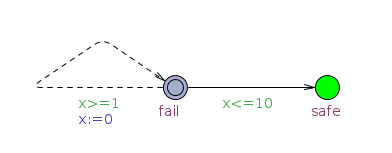
\includegraphics[width=0.8\textwidth]{picture/tiga.png}
    \caption{Basic example made with UPPAAL TiGa}
  \end{center}
\end{figure}
In this example, the environment is represented by the cut lines. We start from the fail state and two different states can be reached. Either we go back to the left state because the environment decided to take his transition and to reset the clock x to 0, either to go to the safe state if the controller decided so. If the controller and the environment want to play at the same time, the environment actually plays.
 \subsection{PRISM}
 PRISM is a probabilistic model checker allowing formal modelling and analysis of systems that exhibit random or probabilistic behaviour. In our case, we will use PRISM to model a Continuous-Time Markov Chain (CTMCs) but there are other models that can be be modeled thanks to this tool. \\
 Thanks to PRISM, we will for example be able to show that every traffic lights will get the green light in an equal and fair way, meaning that there will be no starvation for one of them. Moreover, thanks to PRISM, we can show the statistics of green light possession for every different traffic light, something that is not possible to do in Uppaal. This is why we decided to also rewrite our model in PRISM so new kind of properties could be demonstrated.
 \begin{figure}[h]\label{fig:prism}
  \begin{center}
    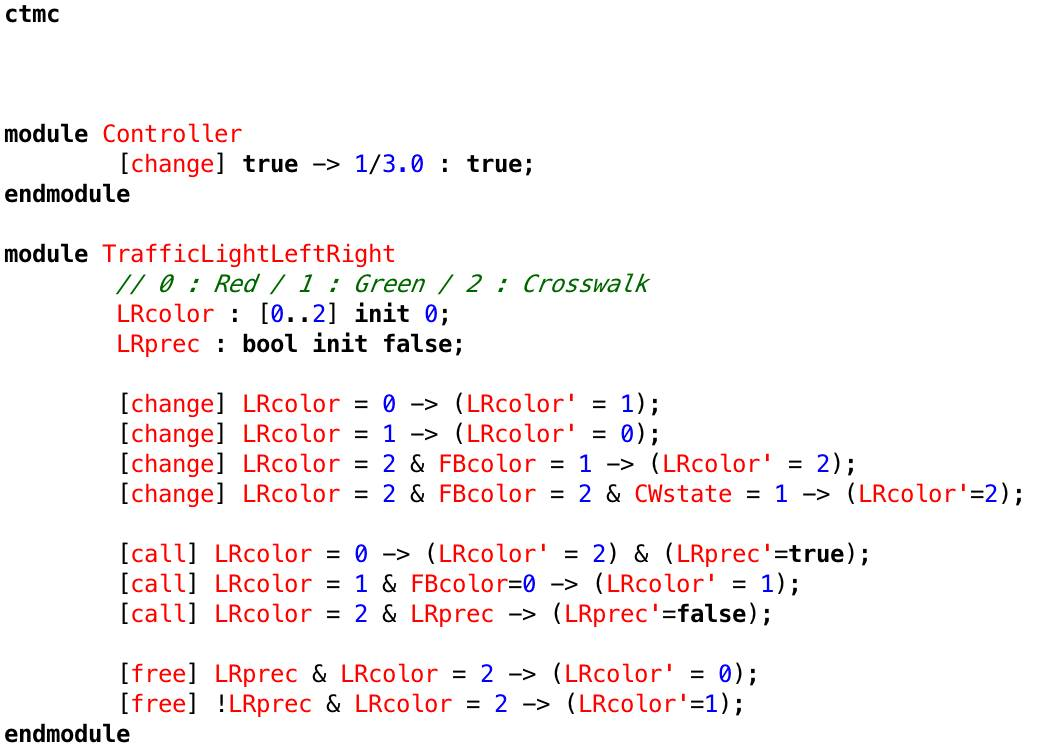
\includegraphics[width=0.8\textwidth]{picture/prism.png}
    \caption{Example of the PRISM language}
  \end{center}
\end{figure} 

\noindent In this basic code, we can already see how the syntax works in PRISM. We first define that our model will follow a Continuous-Time Markov Chain by writing ctmc as first line. We then define what PRISM call \textit{module} and it is the same that what we called \textit{Template} in Uppaal. There, we will define our Controller, our different traffic lights and so on. \\
We can communicate through the different module thanks to the labels we put between brackets and every component with the same label will be executed at the same time, once. \\
One problem with PRISM and our project is that we want the traffic lights to change every T seconds. This is something that cannot really be done in PRISM, at short-term. Indeed, even if we define a rate, systems transitions can still happen even if $T' \ne T $. This will be solved by looking at how our system works in long-term and in a long-run. Indeed, the rate that is defined by our controller will be reach T when the number of executions is high. \\ 
This is why we can use PRISM and we will use it to demonstrate other properties that cannot be shown in Uppaal.

\section{Model Checking}
\subsection{Introduction}
To build our final model, we decided to use an incremental way of construction, meaning that we started from a Minimum Viable Product that we augmented each step. At the end of the day, 4 steps were created. We will now, without entering in the details for the first steps, explain what can be done there. The final step will be deeply explained since it is the most complex one.

\subsubsection{Step 1 - Basic Traffic Lights system}
In this first basic step, we modeled in Uppaal a simple controller sending a pulse every 3 seconds to two cars traffic lights. There is no pedestrians and no buses in this step. \\
Every 3 seconds, the South and North traffic lights switch from green to red while the East and West traffic lights switch, on the opposite, from red to green. \\
Thanks to this basic example, we understood how Uppaal works and how it is possible to send messages from one component to an other component thanks to the channels message passing system. \\
In this system, it is possible to check whether our first traffic light is green and the other is red before a certain time and vice-versa. We also check if we never reach a state where our system is in an impossible state where both traffic lights are green.
\subsubsection{Step 2 - Pedestrians}
In this step, many different things were added to the step 1. Pedestrians were now added and many different things had to be changed to allow this. \\ 
When a pedestrians call was send by the environment, the car's traffic light that was green had to become red and the other car traffic light had to stay red. When those two traffic lights are red, the pedestrians traffic light could be green. Because we also wanted fairness in our system, two assumptions were here created.
\begin{enumerate}
    \item When the pedestrians traffic light is green, we have to remember which car traffic light was previously green. This will be useful for the next assumption.
    \item We wanted fairness between the actors, even if pedestrians have the priority. The problem at the beginning was that starvation could happen if, when the pedestrians lights are green, we always switched to a specific car's traffic light. This would mean that the other car's traffic light would remain red if pedestrians are always calling. We thus added what we called a "delayed" call where, even if the pedestrians are always pressing the button, the two cars lights have to be green at least once before the pedestrians could have their lights green again. This is why the first assumption is useful, we have to remember which car's light was previously green so the cars in the other side of the crossroad don't always have to wait 2 times to be green again. \\
    As an example, if the East-West car's traffic light is green and a pedestrian pressed the button, after the pedestrians lights switch from green to red, the North-South car's traffic light is switched to green so they do not have to wait another time.
\end{enumerate}
In this step, more properties were checked. We for example check if, after a transition, the value of a component always reaches the enquired value. We also check, as for the first one, that certain states can never be reached in our model (all traffic lights are green for example).

\subsubsection{Step 3 - Buses}
In this step, we added the buses generated by the environment. The idea here is that the buses have total priority on the pedestrians and the the cars, as it is the case in Belgium for example. \\
When a bus is generated, the next traffic light that has to be green is the one of the bus. When the bus is crossing, all other lights are green because the bus will go through all the crossroad. \\
Even if the pedestrians have called to have the green lights before the bus, if a bus is generated between the call and the pedestrians green light, we will first give the green light for the bus, then the pedestrians, then the cars. This mean that the priority hierarchy is \textit{Buses-Pedestrians-Cars}. 

\subsubsection{Step 4 - Yellow Light}
For this step, we kept the same model done in step 3 but we added a yellow light. This means that, as in the real life, our cars traffic lights will switch from green to yellow to red. \\
This is thus our final model developed in Uppaal TiGa.

\subsection{Timed Automatons}
In order to formally model the system, we use several timed automatons from Uppaal. While some of those automatons are actors in the environment, the others are part of the controller.
The theory tells us that, when the environment is playing, we, humans, cannot decide the action that will be taken. For example, buses and pedestrians arrivals are unpredictable and uncontrollable, so they belong to the environment.
The actors which implement the solution for avoiding crashes belong to the controller. They interact with the environment in order to avoid crashes and thus they aim to find a winning strategy.


\subsection{Tested Propreties}
In this section, we will give and explain the code to formally verify that our system is correct. We are going to check :
\begin{itemize}
	\item Safety : unwanted system states are never reached (e.g. conflicting green light),
	\item Liveness : desired behavior eventually happen (e.g. everyone get a green light at some point),
	\item Fairness : infinitely done requests are infinitely satisfied (nobody will have to wait too long).
\end{itemize}

The first two have been checked with Uppaal and the last one with Prism.

\subsubsection{Liveness}
We will first give some liveness properties about our system.
\begin{enumerate}
  \item If a bus has been called, he will never have to wait indefinitely to cross the road. Since our bus can reach several states, we check for each of them if the light will be green at some point. 
  \begin{itemize}
    \item $Bus.DelayedCall --> Bus.Green$ 
    \item $Bus.Preempted --> Bus.Green$
    \item $Bus.Called --> Bus.Green$
  \end{itemize}
  \item If a pedestrian call has been made, they will never have to wait indefinitely to cross the crosswalk. Since our pedestrians can reach several states, we check for each of them if the light will be green at some point. 
  \begin{itemize}
    \item $Crosswalk.DelayedCall --> Crosswalk.Green$ 
    \item $Crosswalk.Preempted --> Crosswalk.Green$
    \item $Crosswalk.Called --> Crosswalk.Green$
  \end{itemize}
  \item No deadlock, meaning that the system will never freeze.
  \begin{itemize}
    \item \textit{A[] not deadlock}
  \end{itemize}
\end{enumerate}
Since we use Uppaal TiGa, there is not only a controller but also an environment. We thus took this into consideration and we wrote some properties about the maximum time one actor of the environment will have to wait.
\begin{enumerate}
  \item The maximum waiting time for a pedestrian is at most 3P (meaning 3 times the period we have chosen). Indeed, if he has just been called recently, he will have to wait 2P and if a bus has been called before, we have to give him the priority and wait 1P.
  \begin{itemize}
    \item \textit{A[] not( Crosswalk.Green \&\& Crosswalk.ct>4*P)}
    \item We here have to put 4P because the light will stay green until the end of the fourth green light
  \end{itemize}
  \item The maximum waiting time for a bus is at most 2P. Indeed, if he has just been called recently, he will have to wait 2P since the bus has the priority.
  \begin{itemize}
    \item \textit{A[] not( Bus.Green \&\& Bus.bt>3*P )}
    \item We here have to put 3P because the light will stay green until the end of the third green light
  \end{itemize}
  \item The cars traffich lights will be green again before 4P.
  \begin{itemize}
    \item \textit{A[] not( TrafficLightFrontBack.Green \&\& TrafficLightFrontBack.tlfbc>4*P )}
    \item \textit{A[] not( TrafficLightLeftRight.Green \&\& TrafficLightLeftRight.tllrc>4*P )}
  \end{itemize}
\end{enumerate}
\subsubsection{Safety} 
On the opposite of the first proprety we defined, the liveness one, we will here not try to find that something willeventually happen. We will here show that some events will \textbf{never} happen because if it was the case, we would reach incoherent states leading to a failure in our system. In our traffic light model, it would means that two opposite actors could cross the crossroad at the same time, leading to a crash. 
\begin{enumerate}
  \item We check that if the crosswalk light is green, no other lights can be green at the same time.
  \begin{itemize}
    \item \textit{A[] not (((Crosswalk.Green or Crosswalk.Free) and  (Bus.Green or Bus.Free)) or ((Crosswalk.Green or Crosswalk.Free) and TrafficLightFrontBack.Green) or ((Crosswalk.Green or Crosswalk.Free) and TrafficLightLeftRight.Green))}
    \item Since we consider in our model that the Free state is still a green state, we have to check for both of those states.
  \end{itemize}
  \item We check that if the bus's light is green, no other lights can be green at the same time.
  \begin{itemize}
    \item \textit{A[] not (((Bus.Green or Bus.Free) and  (Crosswalk.Green or Crosswalk.Free)) or ((Bus.Green or Bus.Free) and TrafficLightFrontBack.Green) or ((Bus.Green or Bus.Free) and TrafficLightLeftRight.Green))}
  \end{itemize}
  \item If the car FrontBack traffic light is green, no other lights can be green.
  \begin{itemize}
    \item \textit{A[] not ( (TrafficLightFrontBack.Green and (Bus.Green or Bus.Free)) or (TrafficLightFrontBack.Green and (Crosswalk.Green or Crosswalk.Free)) or (TrafficLightFrontBack.Green and TrafficLightLeftRight.Green))}
  \end{itemize}
  \item If the car LeftRight traffic light is green, no other lights can be green.
  \begin{itemize}
    \item \textit{A[] not ( (TrafficLightLeftRight.Green and (Bus.Green or Bus.Free)) or (TrafficLightLeftRight.Green and (Crosswalk.Green or Crosswalk.Free)) or (TrafficLightLeftRight.Green and TrafficLightFrontBack.Green))}
  \end{itemize}
\end{enumerate}
Thanks to those properties, we could reach a winning strategy where, even if our environment plays, everything will be under control and unfortunate situations will be avoided. In our case, it means that our crosswalk is working the way we want it to work and we were able to prove it thanks to the Verifier from Uppaal.

\subsubsection{Fairness} \label{verif:fairness}

This properties has been checked in PRISM

\paragraph{Crosswalk}

Here we show that our three traffic lights are green with almost the same percentage of time. This can be seen on Figure \ref{fig:prism1}. On this graph, the X-axis represent the average time elapsed between two crosswalk calls while the Y-axis represent the number of times a traffic light is switching to the green state every T (300 in our case) units of time. What we can see is that the more time there is between the pedestrians call, the more our car traffic lights will remain green.

\begin{figure}[H]\label{fig:prism1}
  \centering
    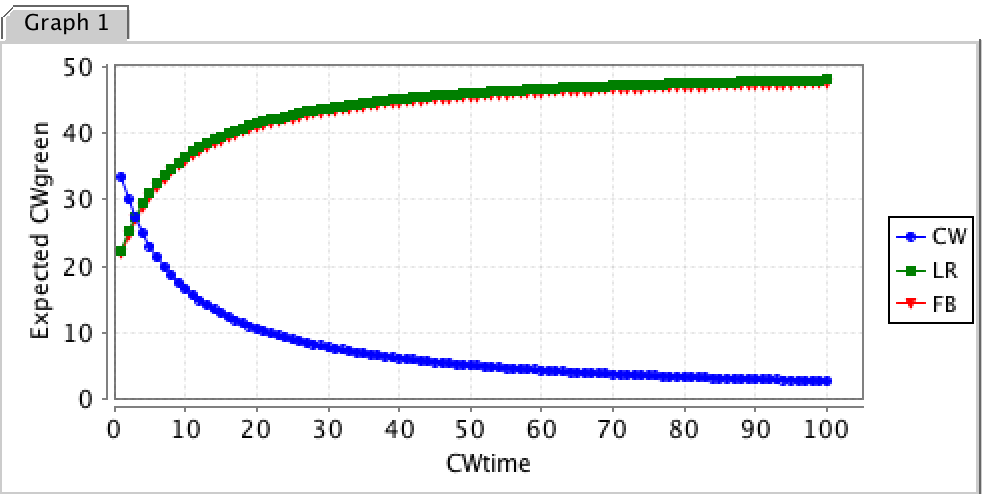
\includegraphics[width=0.5\textwidth]{picture/graphprism.png}
    \caption{Percentage of green lights between the traffic lights}
\end{figure}

\paragraph{Crosswalk and buses}

Here we obtain more specific details about our implementation. For example, we calculate the effect of the time that has elapsed between two buses with as constant the time of a pedestrian call. We also look at the effect of the time between two pedestrians on the green light of the bus for different time between two buses. \\

We choose to have only one dependent variable for each of the graph and fixed the value of the independent variable.
\begin{itemize}
	\item FB : the light for the car in the north-south direction,
	\item LR : the light for the car in the east-west direction,
	\item CW : the light for the pedestrians,
	\item BUS : the light for the bus.
\end{itemize}


\begin{figure}[H]\label{fig:cwfirst}
  \centering
    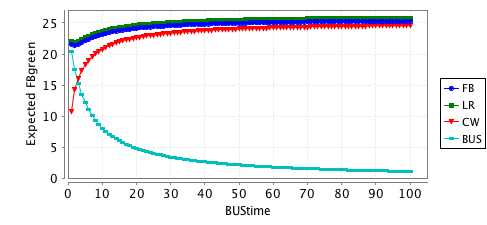
\includegraphics[width=0.5\textwidth]{picture/CWtime1.png}
    \caption{Effect of time that has elapsed between two buses with pedestrian call = 1 unit of time}
\end{figure}

\begin{figure}[H]\label{fig:cwthree}
  \centering
    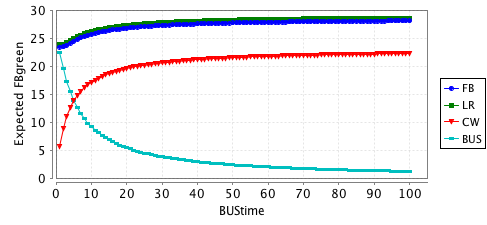
\includegraphics[width=0.5\textwidth]{picture/CWtime3.png}
    \caption{Effect of time that has elapsed between two buses with pedestrian call = 3 units of time}
\end{figure}

\begin{figure}[H]\label{fig:busbus}
  \centering
    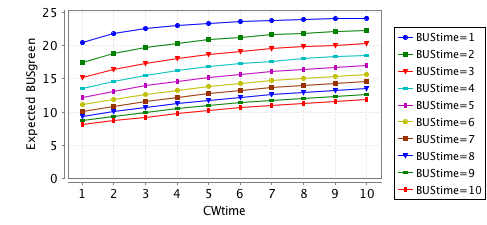
\includegraphics[width=0.5\textwidth]{picture/CWtimeOnBUS.png}
    \caption{Effect of the time between two pedestrians calls on the bus green light}
\end{figure}

Those details can be seen on Figure 4.4, 4.5 and 4.6.
\section{Conclusion}
Thanks to this project, we now have a better understanding of what is formal verification and how it is possible to do it. We experimented the development of a system driven by model checking. \\
The problem in those kind of models is to be able to identify the main issues that could happen in the real world and to write the properties related to it. The second difficulty is to write the correct automatons related to those real models but thanks to those automatons, a lot of useful properties could be defined and verified.\\
Model checking helps us to be sure that our system is correct, if the model is correct of course. If it is not the case, model checking helps us to highlight what is wrong in the system. 
\end{document}
